% Compile with: pdflatex lenses_figures.tex
%
% TikZ diagrams for the four "lens" feature families implemented in
%   SRC/lens_features_extractor.py
% (NLF, CFA, residual-spectrum [radial+angular], LCA).
%
% Each figure stands alone; the first one summarises the whole pipeline.

\documentclass[11pt]{article}
\usepackage[a4paper, margin=22mm]{geometry}
\usepackage{tikz}
\usepackage{amsmath, amssymb}
\usepackage{booktabs}
\usepackage{pgfplots}
\pgfplotsset{compat=1.18}
\usetikzlibrary{
  arrows.meta,
  positioning,
  fit,
  backgrounds,
  calc,
  shapes.geometric,
  decorations.pathreplacing,
  matrix
}

% --- shared styles --------------------------------------------------------
\tikzset{
  block/.style    = {draw, rounded corners=2pt, align=center,
                     inner sep=4pt, minimum height=8mm, font=\small},
  data/.style     = {draw, rectangle, rounded corners=1pt,
                     fill=blue!8, align=center, font=\small\ttfamily,
                     inner sep=3pt},
  feat/.style     = {draw, rectangle, fill=orange!15, align=center,
                     font=\small\ttfamily, inner sep=3pt},
  proc/.style     = {draw, rectangle, fill=gray!8, align=center,
                     font=\small, inner sep=3pt},
  arrow/.style    = {-{Latex[length=2mm]}, thick},
  thinarrow/.style= {-{Latex[length=1.6mm]}, semithick},
  note/.style     = {font=\scriptsize\itshape, text=black!60},
}

\title{Forensic ``lenses'' --- diagrammatic summary}
\author{ADAIS / wave\_1}
\date{}

\begin{document}
\maketitle

\noindent
\textbf{Source.}
\texttt{SRC/lens\_features\_extractor.py}.  Four pure-numpy feature families
that target \emph{positive camera provenance} (capture-time physical traces)
rather than absence of generative artefacts.

\paragraph{Block budget (default config).}
\begin{center}
\small
\begin{tabular}{lcl}
\toprule
Block & dim & contents \\
\midrule
NLF                       & 20 & 16 curve bins $+$ \{a, b, $R^2$, valid\_frac\}\\
CFA                       & 12 & 3 channels $\times$ \{peak\_hh, vh, dh, pool\}\\
RES, radial spectrum      & 64 & log-spaced radial bins, L1-normalised\\
RES, angular spectrum     & 16 & sectors of $11.25^{\circ}$ in $[0,\pi)$\\
LCA                       &  8 & 2 pairs (R$\to$G, B$\to$G) $\times$ \{slope, $R^2$, mean\_tan, std\_rad\}\\
\midrule
\textbf{total}            & \textbf{120} & \\
\bottomrule
\end{tabular}
\end{center}

\bigskip

% =========================================================================
\section*{1. Pipeline overview}
% =========================================================================

\begin{figure}[h]
\centering
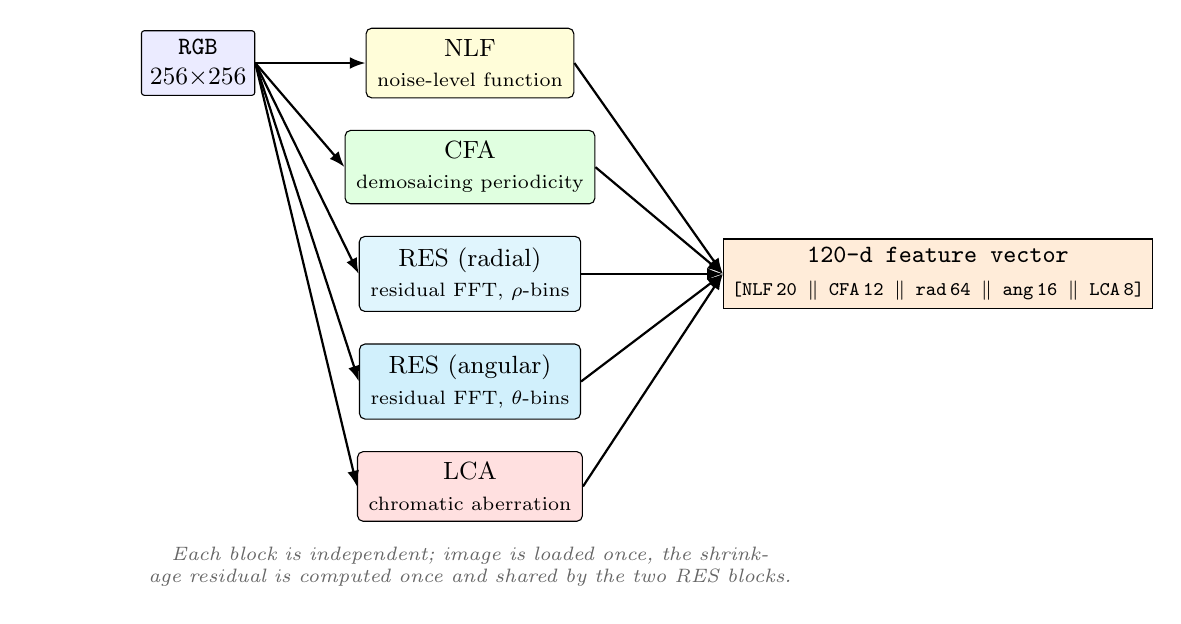
\begin{tikzpicture}[node distance=8mm and 11mm]

\node[data] (img) {RGB \\ $256{\times}256$};

\node[block, right=14mm of img, fill=yellow!15] (nlf) {NLF\\ \scriptsize noise-level function};
\node[block, below=4mm of nlf, fill=green!12]   (cfa) {CFA\\ \scriptsize demosaicing periodicity};
\node[block, below=4mm of cfa, fill=cyan!12]    (rrad){RES (radial)\\ \scriptsize residual FFT, $\rho$-bins};
\node[block, below=4mm of rrad,fill=cyan!18]    (rang){RES (angular)\\ \scriptsize residual FFT, $\theta$-bins};
\node[block, below=4mm of rang,fill=red!12]     (lca) {LCA\\ \scriptsize chromatic aberration};

\node[feat, right=18mm of rrad, minimum width=42mm] (out) {\textbf{120-d feature vector}\\[1pt]
  \scriptsize [NLF\,20 $\Vert$ CFA\,12 $\Vert$ rad\,64 $\Vert$ ang\,16 $\Vert$ LCA\,8]};

\foreach \n in {nlf,cfa,rrad,rang,lca}{
  \draw[arrow] (img.east) -- (\n.west);
  \draw[arrow] (\n.east) -- (out.west);
}

\node[note, below=2mm of lca, align=center, text width=110mm]
  {Each block is independent; image is loaded once, the shrinkage residual
   is computed once and shared by the two RES blocks.};
\end{tikzpicture}
\caption{Top-level layout. The image enters once; five lenses run in
parallel and their outputs are concatenated.}
\end{figure}

\clearpage
% =========================================================================
\section*{2. NLF --- Noise-Level Function}
% =========================================================================

\noindent
\emph{Idea.} A real sensor produces \emph{heteroscedastic} noise
$\sigma^2(I) = aI + b$ (Poisson--Gaussian). AR/diffusion decoders do not.

\begin{figure}[h]
\centering
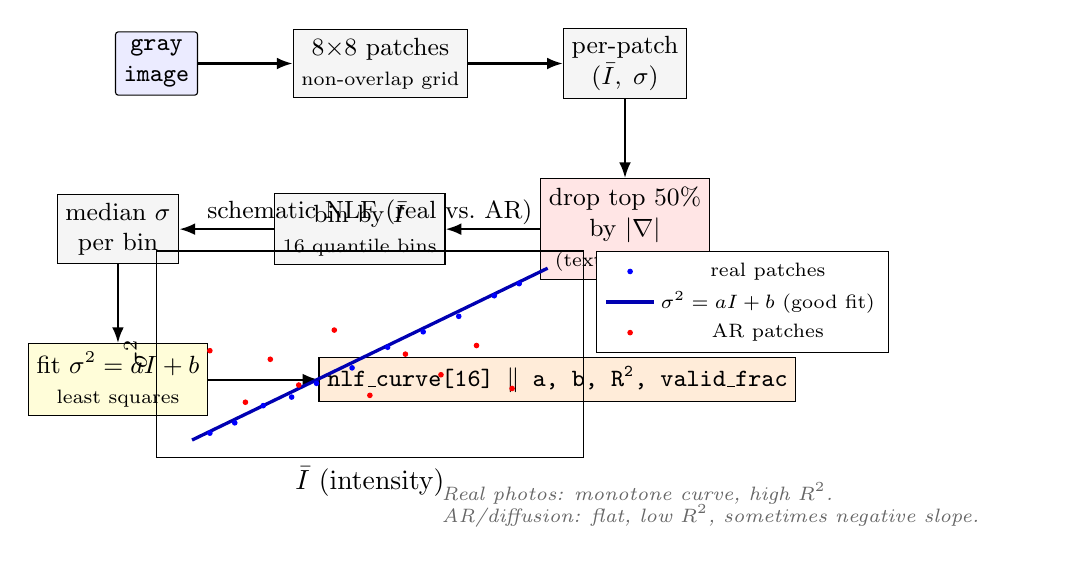
\begin{tikzpicture}[node distance=10mm and 12mm]

\node[data] (gray) {gray\\ image};
\node[proc, right=of gray] (patches) {$8{\times}8$ patches\\ \scriptsize non-overlap grid};
\node[proc, right=of patches] (ms) {per-patch\\ $(\bar I,\;\sigma)$};
\node[proc, below=of ms, fill=red!10] (drop)
   {drop top 50\%\\ by $|\nabla|$\\ \scriptsize (texture filter)};
\node[proc, left=of drop] (bin) {bin by $\bar I$\\ \scriptsize 16 quantile bins};
\node[proc, left=of bin] (med)  {median $\sigma$\\ per bin};

\node[proc, below=of med, fill=yellow!15] (fit)
   {fit $\sigma^2 = aI + b$\\ \scriptsize least squares};

\node[feat, right=14mm of fit, minimum width=58mm]
   (out) {\texttt{nlf\_curve[16]} $\Vert$ \texttt{a, b, R\textsuperscript{2}, valid\_frac}};

\draw[arrow] (gray) -- (patches);
\draw[arrow] (patches) -- (ms);
\draw[arrow] (ms) -- (drop);
\draw[arrow] (drop) -- (bin);
\draw[arrow] (bin) -- (med);
\draw[arrow] (med) -- (fit);
\draw[arrow] (fit) -- (out);

% schematic scatter / fit
\begin{scope}[shift={(0,-5.0)}]
  \begin{axis}[
      width=70mm, height=42mm,
      xlabel={$\bar I$ (intensity)}, ylabel={$\sigma^2$},
      xtick=\empty, ytick=\empty,
      title={\small schematic NLF (real vs.\ AR)},
      legend pos=outer north east, legend style={font=\scriptsize},
      enlargelimits=true,
    ]
    % real: linear w/ scatter
    \addplot+[only marks, mark size=0.8pt, mark options={fill=blue,draw=blue}]
      coordinates{(0.05,0.012)(0.12,0.018)(0.20,0.028)(0.28,0.033)
                  (0.35,0.041)(0.45,0.050)(0.55,0.062)(0.65,0.071)
                  (0.75,0.080)(0.85,0.092)(0.92,0.099)};
    \addlegendentry{real patches}
    \addplot+[domain=0:1, samples=2, very thick, blue!70!black, no marks]{0.10*x+0.008};
    \addlegendentry{$\sigma^2=aI+b$ (good fit)}
    % AR: flat/unstructured
    \addplot+[only marks, mark size=0.8pt, mark options={fill=red,draw=red}]
      coordinates{(0.05,0.060)(0.15,0.030)(0.22,0.055)(0.30,0.040)
                  (0.40,0.072)(0.50,0.034)(0.60,0.058)(0.70,0.046)
                  (0.80,0.063)(0.90,0.038)};
    \addlegendentry{AR patches}
  \end{axis}
\end{scope}

\node[note, anchor=north west] at (3.5,-5.2)
   {\parbox{75mm}{Real photos: monotone curve, high $R^2$.\\
                  AR/diffusion: flat, low $R^2$, sometimes negative slope.}};
\end{tikzpicture}
\caption{NLF block. Patches are filtered for content, binned by mean
intensity, and the resulting $(\bar I,\sigma)$ curve is fit to the
Poisson--Gaussian model. The fit residuals are themselves informative.}
\end{figure}

\clearpage
% =========================================================================
\section*{3. CFA --- Colour Filter Array periodicity}
% =========================================================================

\noindent
\emph{Idea.} Bayer demosaicing leaves a 2-pixel periodic correlation in
each channel's high-pass residual --- visible as peaks at the
half-Nyquist locations of the 2-D FFT.

\begin{figure}[h]
\centering
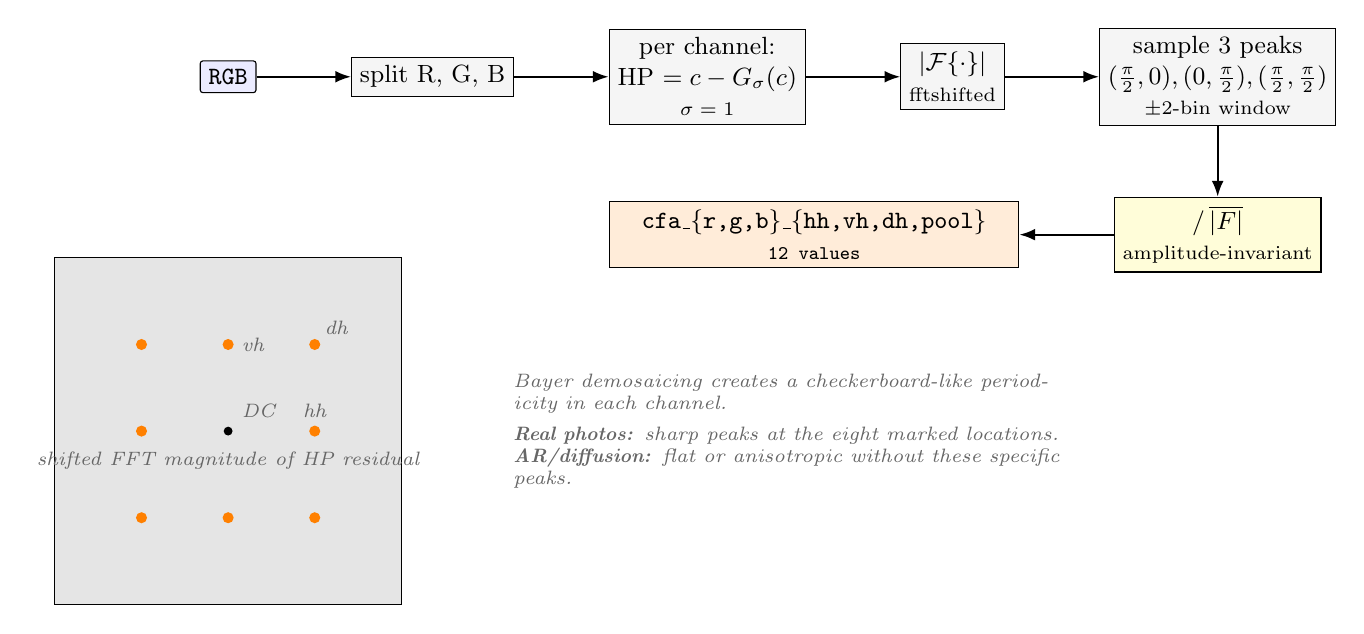
\begin{tikzpicture}[node distance=9mm and 12mm]

\node[data] (rgb) {RGB};
\node[proc, right=of rgb] (split) {split R, G, B};
\node[proc, right=of split] (hp)
   {per channel:\\ HP $= c - G_\sigma(c)$\\ \scriptsize $\sigma=1$};
\node[proc, right=of hp] (fft)  {$|\mathcal{F}\{\cdot\}|$\\ \scriptsize fftshifted};
\node[proc, right=of fft] (peak)
   {sample 3 peaks\\ $(\tfrac{\pi}{2},0),(0,\tfrac{\pi}{2}),(\tfrac{\pi}{2},\tfrac{\pi}{2})$\\
    \scriptsize $\pm 2$-bin window};
\node[proc, below=of peak, fill=yellow!15] (norm)
   {$/\,\overline{|F|}$\\ \scriptsize amplitude-invariant};
\node[feat, left=of norm, minimum width=52mm]
   (out) {\texttt{cfa\_\{r,g,b\}\_\{hh,vh,dh,pool\}}\\ \scriptsize 12 values};

\draw[arrow] (rgb) -- (split);
\draw[arrow] (split) -- (hp);
\draw[arrow] (hp) -- (fft);
\draw[arrow] (fft) -- (peak);
\draw[arrow] (peak) -- (norm);
\draw[arrow] (norm) -- (out);

% schematic spectrum with marked peaks
\begin{scope}[shift={(0,-4.5)}]
  \def\sx{2.2}
  \def\sy{2.2}
  \draw[thick] (-\sx,-\sy) rectangle (\sx,\sy);
  \fill[gray!20] (-\sx,-\sy) rectangle (\sx,\sy);
  % DC
  \fill[black] (0,0) circle (1.6pt);
  \node[note, anchor=south west] at (0.05,0.05) {DC};
  % half-Nyquist locations
  \fill[orange] ( \sx/2, 0) circle (2pt);  \node[note, above] at ( \sx/2, 0.05) {hh};
  \fill[orange] (-\sx/2, 0) circle (2pt);
  \fill[orange] (0,  \sy/2) circle (2pt);  \node[note, right] at (0.05,  \sy/2) {vh};
  \fill[orange] (0, -\sy/2) circle (2pt);
  \fill[orange] ( \sx/2,  \sy/2) circle (2pt); \node[note, above right] at ( \sx/2, \sy/2) {dh};
  \fill[orange] (-\sx/2, -\sy/2) circle (2pt);
  \fill[orange] ( \sx/2, -\sy/2) circle (2pt);
  \fill[orange] (-\sx/2,  \sy/2) circle (2pt);
  \node[note] at (0,-\sy-3mm) {shifted FFT magnitude of HP residual};
\end{scope}

\node[note, anchor=west, text width=70mm] at (3.5,-4.5)
   {Bayer demosaicing creates a checkerboard-like periodicity in each
    channel.\\[3pt]
    \textbf{Real photos:} sharp peaks at the eight marked locations.\\
    \textbf{AR/diffusion:} flat or anisotropic without these specific peaks.};
\end{tikzpicture}
\caption{CFA block. Each of $\{R,G,B\}$ is high-passed, FFT-magnitudes are
sampled at the three half-Nyquist diagnostic frequencies, and normalised
by the mean spectrum to make the score robust to overall residual energy.}
\end{figure}

\clearpage
% =========================================================================
\section*{4. RES --- residual spectrum (radial \& angular)}
% =========================================================================

\noindent
\emph{Idea.} The shrinkage residual (wavelet, by default) of a real photo
has a smooth, monotone fall-off in frequency. Decoder up-sampling kernels
leave periodic replicas: \textbf{radial bins} surface their presence,
\textbf{angular bins} surface their orientation (each generator's
up-sampler has a different signature).

\begin{figure}[h]
\centering
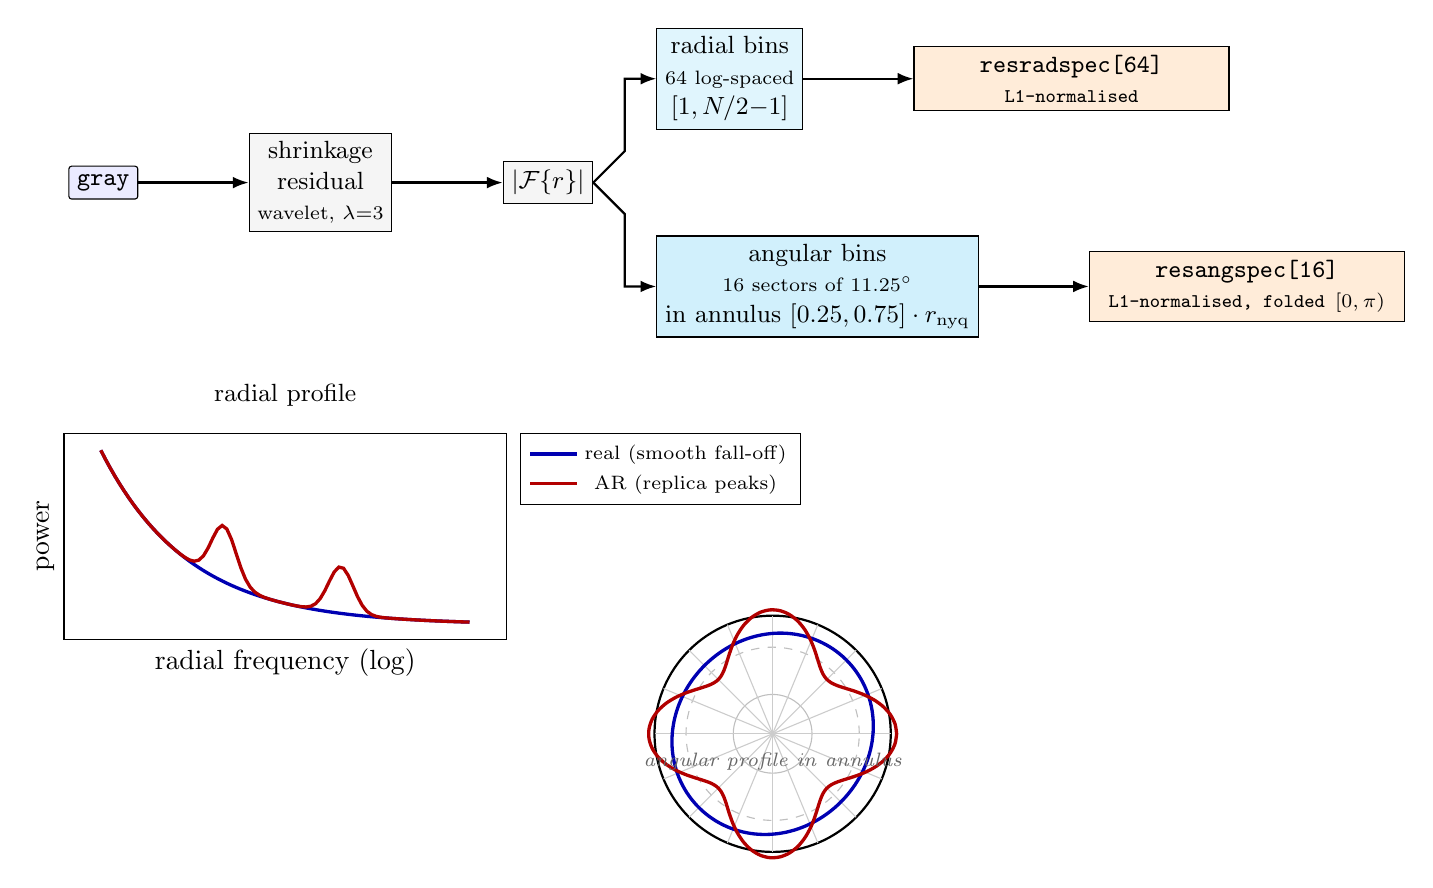
\begin{tikzpicture}[node distance=10mm and 14mm]

\node[data] (gray) {gray};
\node[proc, right=of gray] (res)
   {shrinkage\\ residual\\ \scriptsize wavelet, $\lambda{=}3$};
\node[proc, right=of res] (fft) {$|\mathcal{F}\{r\}|$};

\node[proc, above right=4mm and 8mm of fft, fill=cyan!12] (rad)
   {radial bins\\ \scriptsize 64 log-spaced\\ $[1,N/2{-}1]$};
\node[proc, below right=4mm and 8mm of fft, fill=cyan!18] (ang)
   {angular bins\\ \scriptsize 16 sectors of $11.25^{\circ}$\\
    in annulus $[0.25,0.75]\cdot r_{\text{nyq}}$};

\node[feat, right=of rad, minimum width=40mm]
   (oRad) {\texttt{resradspec[64]}\\ \scriptsize L1-normalised};
\node[feat, right=of ang, minimum width=40mm]
   (oAng) {\texttt{resangspec[16]}\\ \scriptsize L1-normalised, folded $[0,\pi)$};

\draw[arrow] (gray) -- (res);
\draw[arrow] (res)  -- (fft);
\draw[arrow] (fft.east) -- ($(fft.east)+(4mm,4mm)$) |- (rad.west);
\draw[arrow] (fft.east) -- ($(fft.east)+(4mm,-4mm)$) |- (ang.west);
\draw[arrow] (rad) -- (oRad);
\draw[arrow] (ang) -- (oAng);

% small schematic: radial profile (real vs AR)
\begin{scope}[shift={(-0.5,-5.8)}]
  \begin{axis}[
      width=72mm, height=42mm,
      xlabel={radial frequency (log)}, ylabel={power},
      xtick=\empty, ytick=\empty,
      title={\small radial profile},
      legend pos=outer north east, legend style={font=\scriptsize},
    ]
    \addplot[domain=1:64, samples=80, very thick, blue!70!black]
      {0.04*exp(-x/15)};
    \addlegendentry{real (smooth fall-off)}
    \addplot[domain=1:64, samples=80, very thick, red!70!black]
      {0.04*exp(-x/15) + 0.012*exp(-((x-22)/3)^2) + 0.010*exp(-((x-42)/3)^2)};
    \addlegendentry{AR (replica peaks)}
  \end{axis}
\end{scope}

% small schematic: angular polar
\begin{scope}[shift={(8.5,-7.0)}]
  \def\R{1.5}
  \draw[thick] (0,0) circle (\R);
  \draw[gray!50] (0,0) circle (0.5);
  \draw[gray!50,dashed] (0,0) circle (1.1);
  \foreach \a in {0,22.5,...,337.5}{
    \draw[gray!40] (0,0) -- (\a:\R);
  }
  % real: roughly isotropic
  \draw[blue!70!black, very thick]
    plot[domain=0:360,samples=80,smooth]
    ({(\R*0.85 + 0.05*sin(2*\x))*cos(\x)},
     {(\R*0.85 + 0.05*sin(2*\x))*sin(\x)});
  % AR: lobed (e.g. 4-fold)
  \draw[red!70!black, very thick]
    plot[domain=0:360,samples=80,smooth]
    ({(\R*0.85 + 0.30*cos(4*\x))*cos(\x)},
     {(\R*0.85 + 0.30*cos(4*\x))*sin(\x)});
  \node[note] at (0,-\R-3mm) {angular profile in annulus};
\end{scope}
\end{tikzpicture}
\caption{RES block. The same FFT magnitude is binned two ways: radial
bins (top) on a log scale cover the full Nyquist range and discriminate
\emph{real vs.\ synthetic}; angular bins (bottom) live in a mid-frequency
annulus and discriminate \emph{synthetic vs.\ synthetic} via the
orientation pattern of each decoder's up-sampler.}
\end{figure}

\clearpage
% =========================================================================
\section*{5. LCA --- Lateral Chromatic Aberration}
% =========================================================================

\noindent
\emph{Idea.} A real lens refracts wavelengths slightly differently, so the
R and B channels are shifted radially outward from the optical centre.
The shift grows linearly with distance from the centre. AR generators
have no such physics.

\begin{figure}[h]
\centering
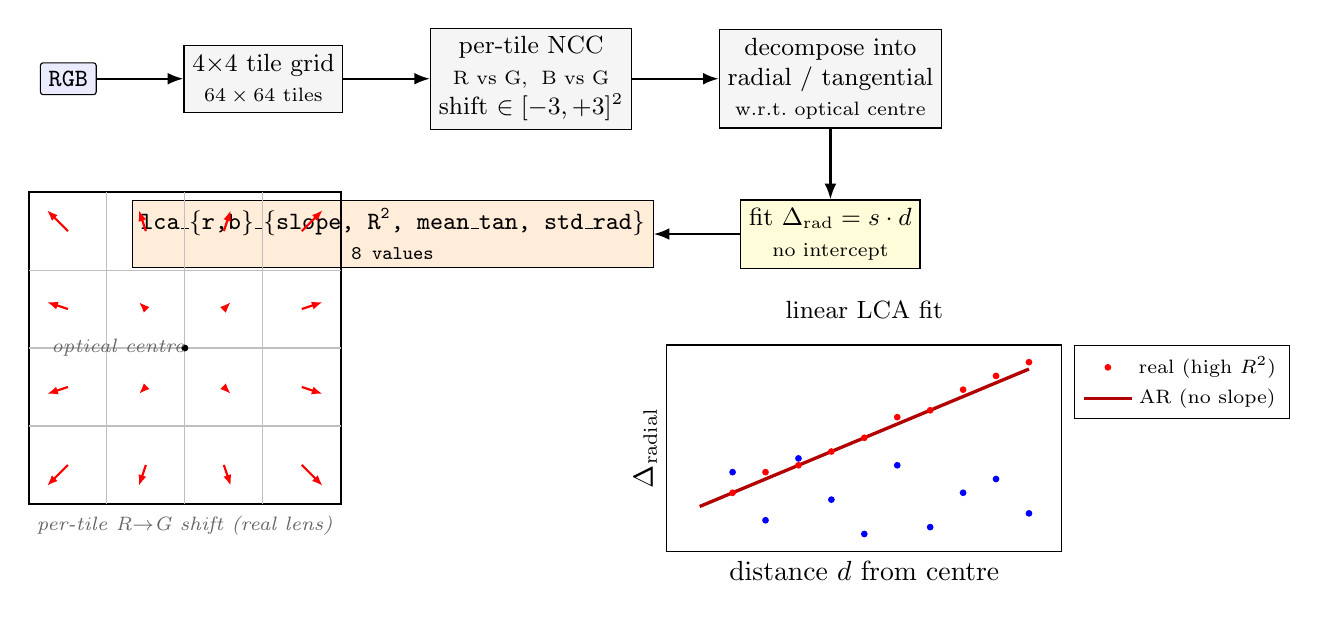
\begin{tikzpicture}[node distance=9mm and 11mm]

\node[data] (rgb) {RGB};
\node[proc, right=of rgb] (grid)
   {$4{\times}4$ tile grid\\ \scriptsize $64\times64$ tiles};
\node[proc, right=of grid] (xc)
   {per-tile NCC\\ \scriptsize R vs G,\; B vs G\\ shift $\in [-3,+3]^2$};
\node[proc, right=of xc] (decomp)
   {decompose into\\ radial / tangential\\ \scriptsize w.r.t.\ optical centre};
\node[proc, below=of decomp, fill=yellow!15] (fit)
   {fit $\Delta_{\text{rad}} = s\cdot d$\\ \scriptsize no intercept};

\node[feat, left=of fit, minimum width=60mm]
   (out) {\texttt{lca\_\{r,b\}\_\{slope, R\textsuperscript{2}, mean\_tan, std\_rad\}}\\ \scriptsize 8 values};

\draw[arrow] (rgb)    -- (grid);
\draw[arrow] (grid)   -- (xc);
\draw[arrow] (xc)     -- (decomp);
\draw[arrow] (decomp) -- (fit);
\draw[arrow] (fit)    -- (out);

% schematic: tile grid with shift arrows pointing outward
\begin{scope}[shift={(-0.5,-5.4)}, scale=0.9]
  \def\S{4.4}
  \draw[thick] (0,0) rectangle (\S,\S);
  \foreach \i in {1,2,3}{
    \draw[gray!50] (\S*\i/4,0) -- (\S*\i/4,\S);
    \draw[gray!50] (0,\S*\i/4) -- (\S,\S*\i/4);
  }
  \fill[black] (\S/2,\S/2) circle (1.4pt);
  \node[note, anchor=west] at (\S/2+1mm,\S/2) {optical centre};

  % outward red arrows (R wrt G), magnitudes grow with distance
  \foreach \i in {0,1,2,3}{
    \foreach \j in {0,1,2,3}{
      \pgfmathsetmacro{\cx}{(\i+0.5)*\S/4}
      \pgfmathsetmacro{\cy}{(\j+0.5)*\S/4}
      \pgfmathsetmacro{\dx}{\cx-\S/2}
      \pgfmathsetmacro{\dy}{\cy-\S/2}
      \pgfmathsetmacro{\dist}{sqrt(\dx*\dx+\dy*\dy)}
      \pgfmathtruncatemacro{\nz}{(\dist>0.05) ? 1 : 0}
      \ifnum\nz=1
        \pgfmathsetmacro{\mag}{0.18*\dist}
        \pgfmathsetmacro{\ux}{\dx/\dist*\mag}
        \pgfmathsetmacro{\uy}{\dy/\dist*\mag}
        \draw[red, -{Latex[length=1.4mm]}, thick]
          (\cx,\cy) -- ++(\ux,\uy);
      \fi
    }
  }
  \node[note] at (\S/2,-3mm) {per-tile R$\to$G shift (real lens)};
\end{scope}

% schematic: slope plot
\begin{scope}[shift={(7.6,-6)}]
  \begin{axis}[
      width=66mm, height=42mm,
      xlabel={distance $d$ from centre}, ylabel={$\Delta_{\text{radial}}$},
      xtick=\empty, ytick=\empty,
      title={\small linear LCA fit},
      legend pos=outer north east, legend style={font=\scriptsize},
    ]
    \addplot+[only marks, mark size=1pt, mark options={fill=red,draw=red}]
      coordinates{(0.10,0.02)(0.20,0.05)(0.30,0.06)(0.40,0.08)
                  (0.50,0.10)(0.60,0.13)(0.70,0.14)(0.80,0.17)
                  (0.90,0.19)(1.00,0.21)};
    \addlegendentry{real (high $R^2$)}
    \addplot[domain=0:1,samples=2, very thick, red!70!black]{0.20*x};
    \addplot+[only marks, mark size=1pt, mark options={fill=blue,draw=blue}]
      coordinates{(0.10,0.05)(0.20,-0.02)(0.30,0.07)(0.40,0.01)
                  (0.50,-0.04)(0.60,0.06)(0.70,-0.03)(0.80,0.02)
                  (0.90,0.04)(1.00,-0.01)};
    \addlegendentry{AR (no slope)}
  \end{axis}
\end{scope}
\end{tikzpicture}
\caption{LCA block. R and B channels are aligned to G on a $4{\times}4$
tile grid via integer NCC search; per-tile shifts are decomposed into a
radial component (along the line to the image centre) and a tangential
component. A real lens gives radial shifts that grow linearly with
distance and a near-zero tangential mean.}
\end{figure}

\end{document}
